\subsection{Zernike modes PSFs Clustering}

	\subsubsection{UMAPS}
		
		Before clustering, UMAPS for flattened PSF matrices, flattend LP coefficients matrices and PL intensities are processed. The same configuration is used for the different number of modes.
		
		\begin{table}[h!]
			\centering
			\begin{tabular}{|c|c|c|c|}
				\hline
				\textbf{Dataset type} & \textbf{Number of neighbors} & \textbf{Min distance} & \textbf{Number of components} \\
				\hline
				PSF electric field & 500 & 0.5 & 1000 \\
				\hline
				PSF intensity & 500 & 0.5 & 1000 \\
				\hline
				Pred PSF electric field & 500 & 0.5 & 1000 \\
				\hline
				Pred PSF intensity & 500 & 0.5 & 1000 \\
				\hline
			\end{tabular}
		\caption{UMAP parameter configurations for PSFs}
		\end{table}
		
	
	\subsubsection{Clustering}
		
		Using DBSCAN I create clusters for the UMAP representations. In the tables CDM and CDV are Cluster Density Mean and Cluster Density Variance respectively.
		
		\paragraph{2 Zernike modes}:
		\begin{table}[h!]
			\centering
			\begin{tabular}{|c|c|c|c|c|c|c|}
				\hline
				\textbf{} & \textbf{$\epsilon$} & \textbf{neighbors} & \textbf{Clusters} & \textbf{CDM} & \textbf{CDV} & \textbf{Non noise points}\\
				\hline
				\textbf{Zernike coeffs} & 0.01 & 6 & 1535 & 41.12 & 92.65 & 63130 \\
				\hline
				\textbf{LP coeffs} & 0.99 & 5 & 1470 & 44.00 & 631.91 & 64686 \\
				\hline
				\textbf{PL fluxes} & 34.7 & 5 & 1431 & 45.46 & 739.78 & 65065 \\
				\hline
				\textbf{PSF electric field} & 0.154 & 5 & 1563 & 40.16 & 110.41 & 62774 \\
				\hline
				\textbf{PSF intensity} & 0.155 & 5 & 1517 & 41.61 & 124.37 & 63125 \\
				\hline
				\textbf{Pred PSF ef} & 0.154 & 5 & 1339 & 41.01 & 159.22 & 63202 \\
				\hline
				\textbf{Pred PSF intensity} & 0.154 & 4 & 1497 & 42.40 & 206.78 & 63480 \\
				\hline
			\end{tabular}
		\caption{DBSCAN clustering for 2 Zernike modes datasets}
		\end{table}
		\FloatBarrier
		
		\paragraph{5 Zernike modes}:
		\begin{table}[h!]
			\centering
			\begin{tabular}{|c|c|c|c|c|c|c|}
				\hline
				\textbf{} & \textbf{$\epsilon$} & \textbf{neighbors} & \textbf{Clusters} & \textbf{CDM} & \textbf{CDV} & \textbf{Non noise points}\\
				\hline
				\textbf{Zernike coeffs} & 0.128 & 4 & 1448 & 38.10 & 1204.20 & 55183 \\
				\hline
				\textbf{LP coeffs} & 12.8 & 4 & 1551 & 34.98 & 1109.08 & 54265 \\
				\hline
				\textbf{PL fluxes} & 410 & 4 & 1500 & 35.54 & 1131.51 & 53324 \\
				\hline
				\textbf{PSF electric field} & 0.31 & 4 & 1587 & 29.02 & 862.14 & 46065 \\
				\hline
				\textbf{PSF intensity} & 0.25 & 4 & 1533 & 34.41 & 1033.01 & 52753 \\
				\hline
				\textbf{Pred PSF ef} & 0.15 & 4 & 1364 & 48.16 & 210.10 & 65691 \\
				\hline
				\textbf{Pred PSF intensity} & 0.27 & 3 & 1645 & 24.95 & 1182.07 & 57491 \\
				\hline
			\end{tabular}
		\caption{DBSCAN Clustering for 5 Zernike modes datasets}
		\end{table}
		\FloatBarrier
		
		\paragraph{9 Zernike modes}:
		\begin{table}[h!]
			\centering
			\begin{tabular}{|c|c|c|c|c|c|c|}
				\hline
				\textbf{} & \textbf{$\epsilon$} & \textbf{neighbors} & \textbf{Clusters} & \textbf{CDM} & \textbf{CDV} & \textbf{Non noise points}\\
				\hline
				\textbf{Zernike coeffs} & 0.29 & 4 & 1428 & 30.30 & 953.86 & 43275 \\
				\hline
				\textbf{LP coeffs} & 26 & 4 & 1485 & 28.01 & 889.60 & 43397 \\
				\hline
				\textbf{PL fluxes} & 770 & 3 & 1616 & 31.85 & 1099.66 & 51474 \\
				\hline
				\textbf{PSF electric field} & 0.26 & 4 & 1459 & 30.45 & 894.56 & 44429 \\
				\hline
				\textbf{PSF intensity} & 0.22 & 4 & 1402 & 39.29 & 1205.03 & 55096 \\
				\hline
				\textbf{Pred PSF ef} & 0.235 & 4 & 1460 & 22.28 & 512.15 & 32530 \\
				\hline
				\textbf{Pred PSF intensity} & 0.235 & 4 & 1385 & 30.49 & 851.07 & 42240 \\
				\hline
			\end{tabular}
		\caption{DBSCAN Clustering for 9 Zernike modes datasets}
		\end{table}
		\FloatBarrier
		
		\paragraph{14 Zernike modes}:
		\begin{table}[h!]
			\centering
			\begin{tabular}{|c|c|c|c|c|c|c|}
				\hline
				\textbf{} & \textbf{$\epsilon$} & \textbf{neighbors} & \textbf{Clusters} & \textbf{CDM} & \textbf{CDV} & \textbf{Non noise points}\\
				\hline
				\textbf{Zernike coeffs} & 0.424 & 3 & 1639 & 25.89 & 880.85 & 42439 \\
				\hline
				\textbf{LP coeffs} & 35.5 & 3 & 1445 & 32.26 & 1064.67 & 46626 \\
				\hline
				\textbf{PL fluxes} & 950 & 3 & 1669 & 24.31 & 814.44 & 40577 \\
				\hline
				\textbf{PSF electric field} & 0.25 & 4 & 1607 & 27.05 & 831.31 & 44202 \\
				\hline
				\textbf{PSF intensity} & 0.21 & 4 & 1436 & 36.52 & 1129.68 & 42830 \\
				\hline
				\textbf{Pred PSF ef} & 0.35 & 3 & 1486 & 36.43 & 1214.19 & 54135  \\
				\hline
				\textbf{Pred PSF intensity} & 0.32 & 3 & 1567 & 36.16 & 1221.05 & 56673 \\
				\hline
			\end{tabular}
		\caption{DBSCAN Clustering for 14 Zernike modes datasets}
		\end{table}
		\FloatBarrier
		
		\paragraph{20 Zernike modes}:
		\begin{table}[h!]
			\centering
			\begin{tabular}{|c|c|c|c|c|c|c|}
				\hline
				\textbf{} & \textbf{$\epsilon$} & \textbf{neighbors} & \textbf{Clusters} & \textbf{CDM} & \textbf{CDV} & \textbf{Non noise points}\\
				\hline
				\textbf{Zernike coeffs} & 0.53 & 3 & 1431 & 26.32 & 841.71 & 37668 \\
				\hline
				\textbf{LP coeffs} & 40.05 & 3 & 1558 & 24.44 & 801.25 & 38079 \\
				\hline
				\textbf{PL fluxes} & 1010 & 3 & 1647 & 18.25 & 566.01 & 30067 \\
				\hline
				\textbf{PSF electric field} & 0.25 & 4 & 1621 & 27.86 & 852.32 & 34332 \\
				\hline
				\textbf{PSF intensity} & 0.20 & 4 & 1559 & 31.47 & 986.86 & 49070 \\
				\hline
				\textbf{Pred PSF ef} & 0.33 & 3 & 1524 & 36.46 & 1222.67 & 55567 \\
				\hline
				\textbf{Pred PSF intensity} & 0.32 & 3 & 1643 & 35.18 & 1191.70 & 57810 \\
				\hline
			\end{tabular}
		\caption{DBSCAN Clustering for 20 Zernike modes datasets}
		\end{table}
		\FloatBarrier
		
	\subsubsection{Results}
	
	
		\begin{figure*}[ht!]
			\centering
			\subfloat[Coefficients NMI evolution]{%
				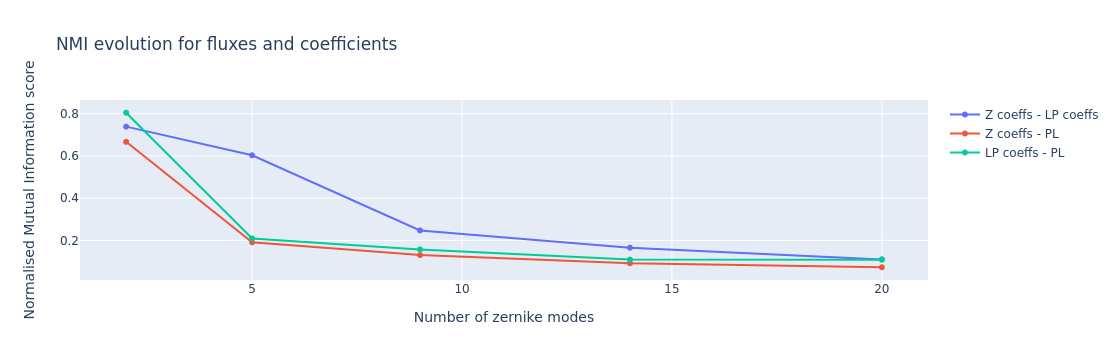
\includegraphics[width=0.45\textwidth]{pid-nmievolutioncoeffs.png}}
			\hspace{\fill}
			\subfloat[PSF to predicted PSF]{%
				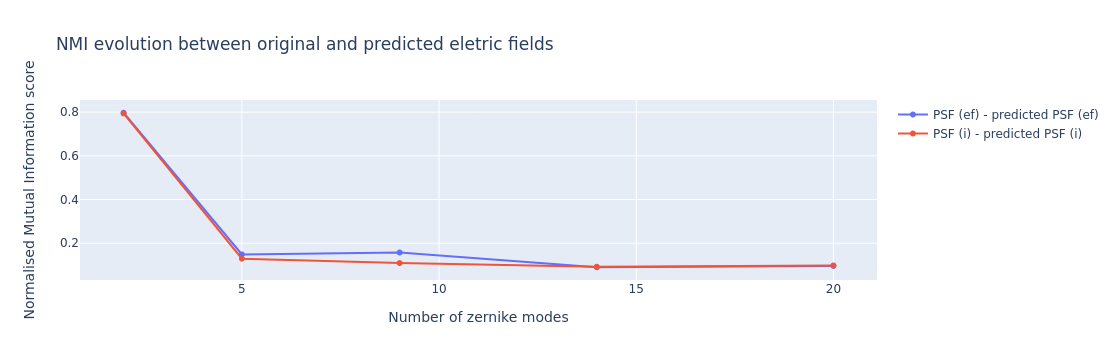
\includegraphics[width=0.45\textwidth]{pid-nmievolutionpsfpredpsf.png}}
			\\
			\subfloat[PSF electric fields to coeffs NMI evolution]{%
				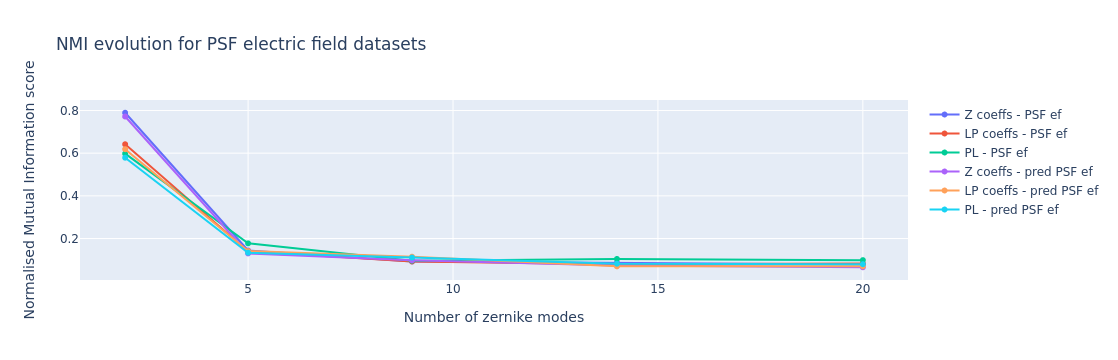
\includegraphics[width=0.45\textwidth]{pid-nmievolutionpsfef.png}}
			\hspace{\fill}
			\subfloat[PSF intenities to coeffs NMI evolution]{%
				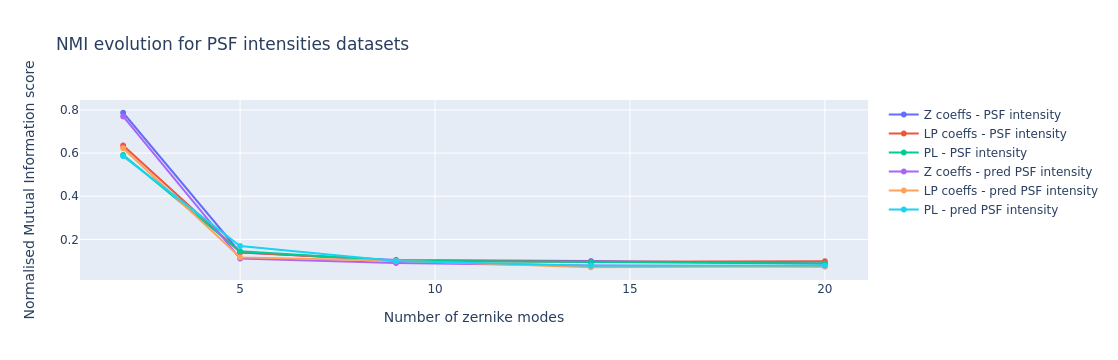
\includegraphics[width=0.45\textwidth]{pid-nmievolutionpsfint.png}}
			\caption{NMI evolution over number of Zernike modes}
		\end{figure*}
		\FloatBarrier
		
		\begin{figure*}[ht!]
			\centering
			\caption{Coefficients NMI}
			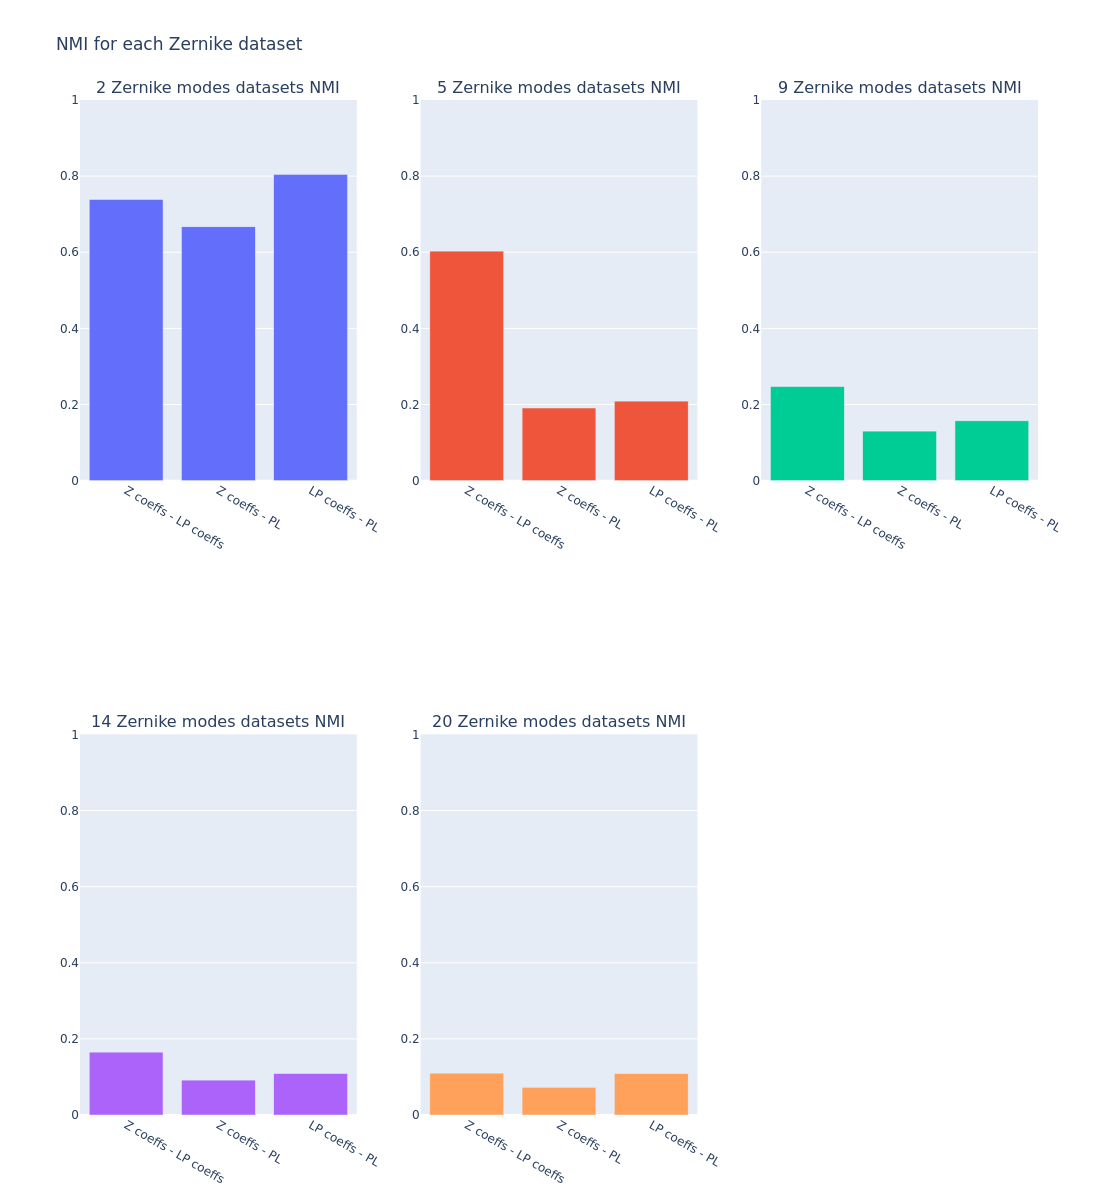
\includegraphics[width=0.9\textwidth]{pid-nmibarcoeffs.png}
		\end{figure*}
		
		\begin{figure*}[ht!]
			\centering
			\caption{PSF electric fields to coeffs NMI evolution}
				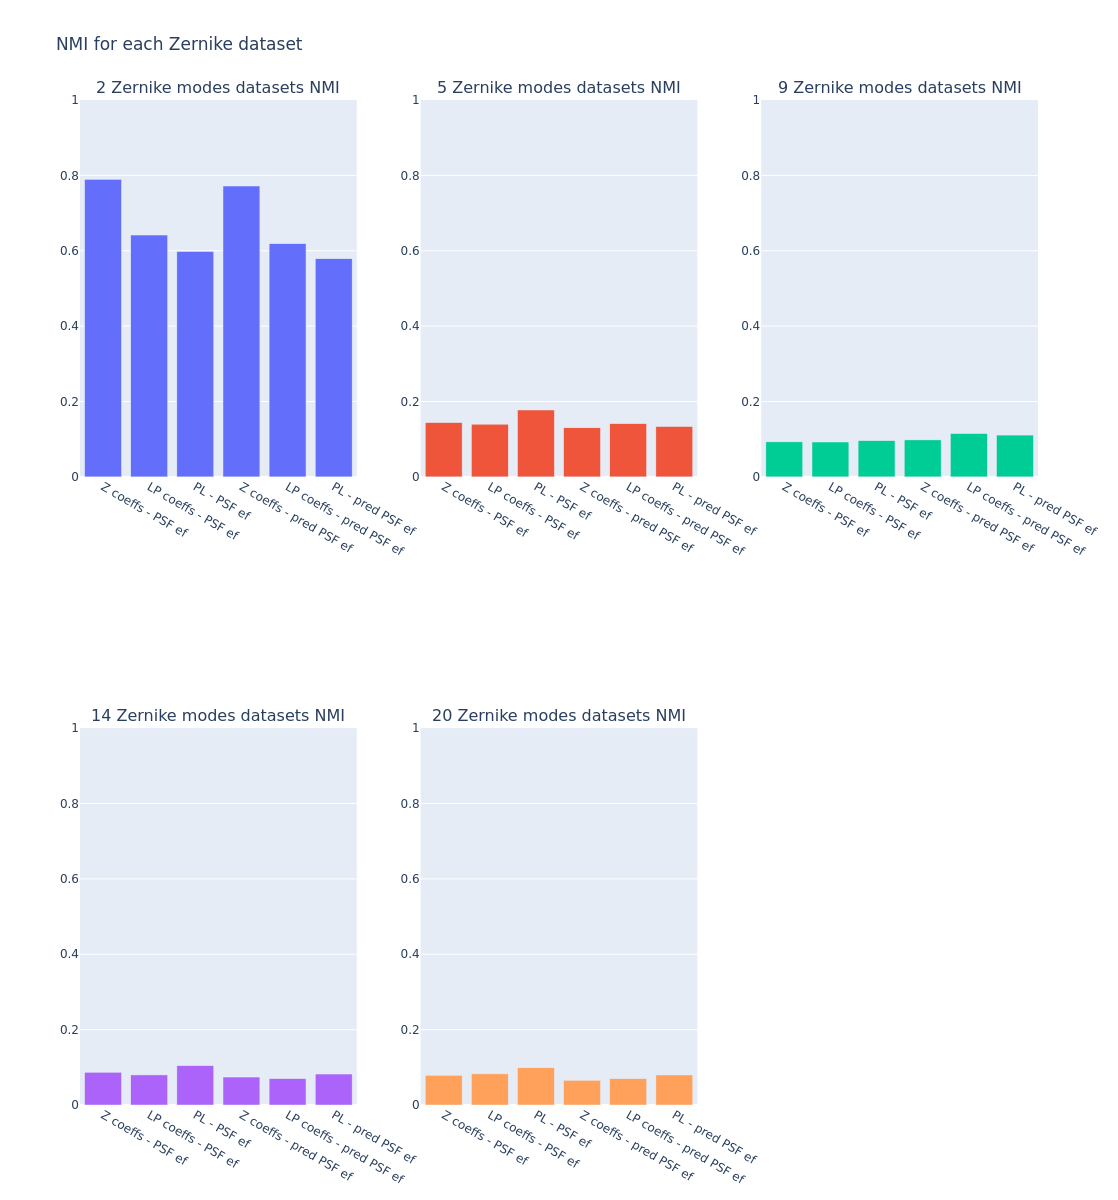
\includegraphics[width=0.9\textwidth]{pid-nmibarpsfef.png}
		\end{figure*}
		
		\begin{figure*}[ht!]
			\centering
			\caption{PSF intensities to coeffs NMI evolution}
				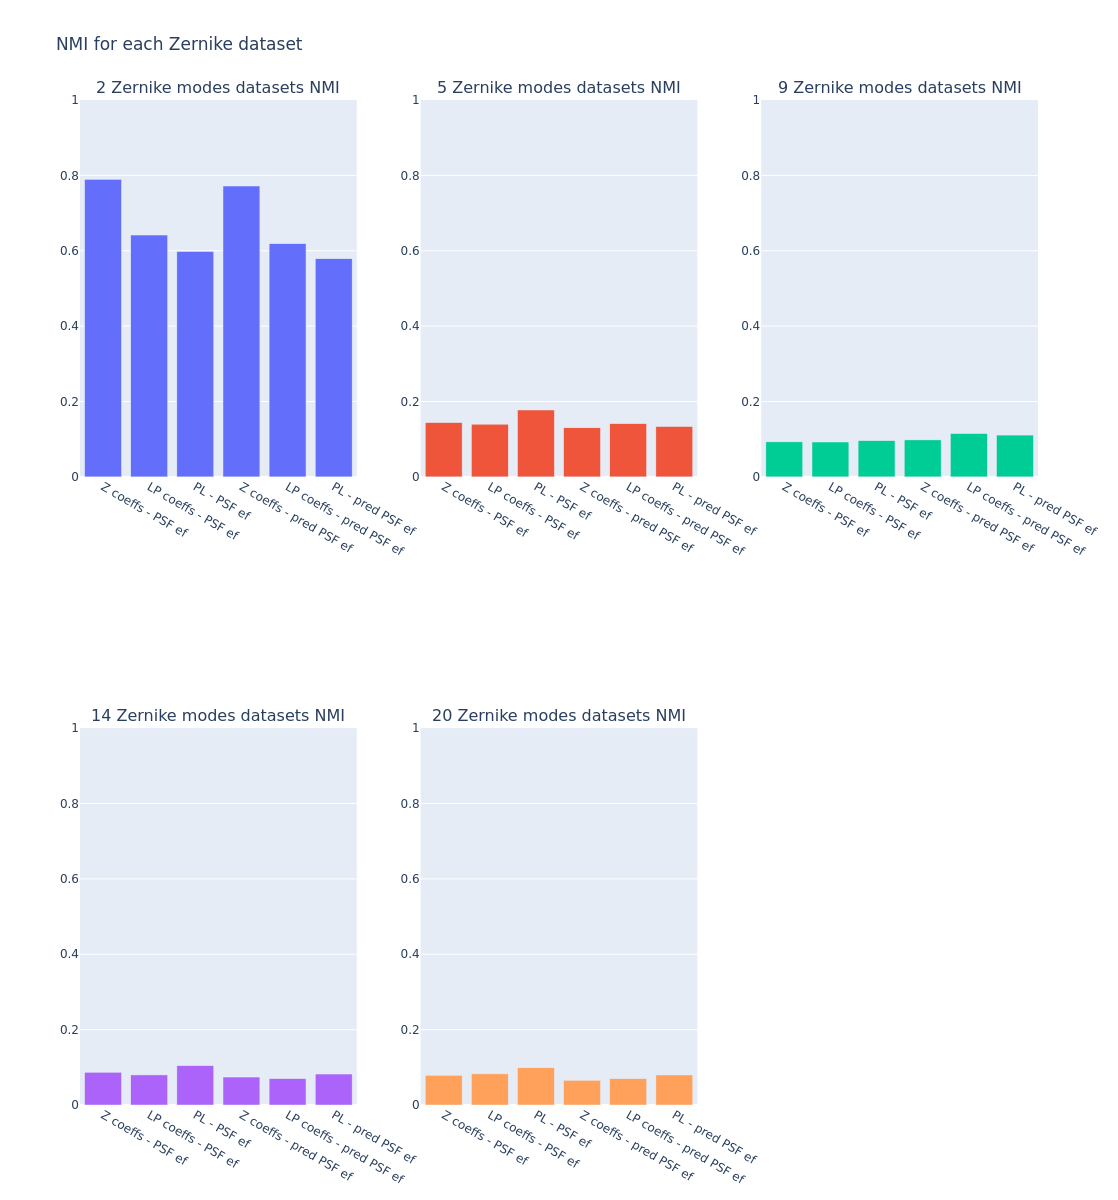
\includegraphics[width=0.9\textwidth]{pid-nmibarpsfint.png}
		\end{figure*}
		
		\begin{figure*}[ht!]
			\centering
			\caption{PSF to predicted PSF NMI}
				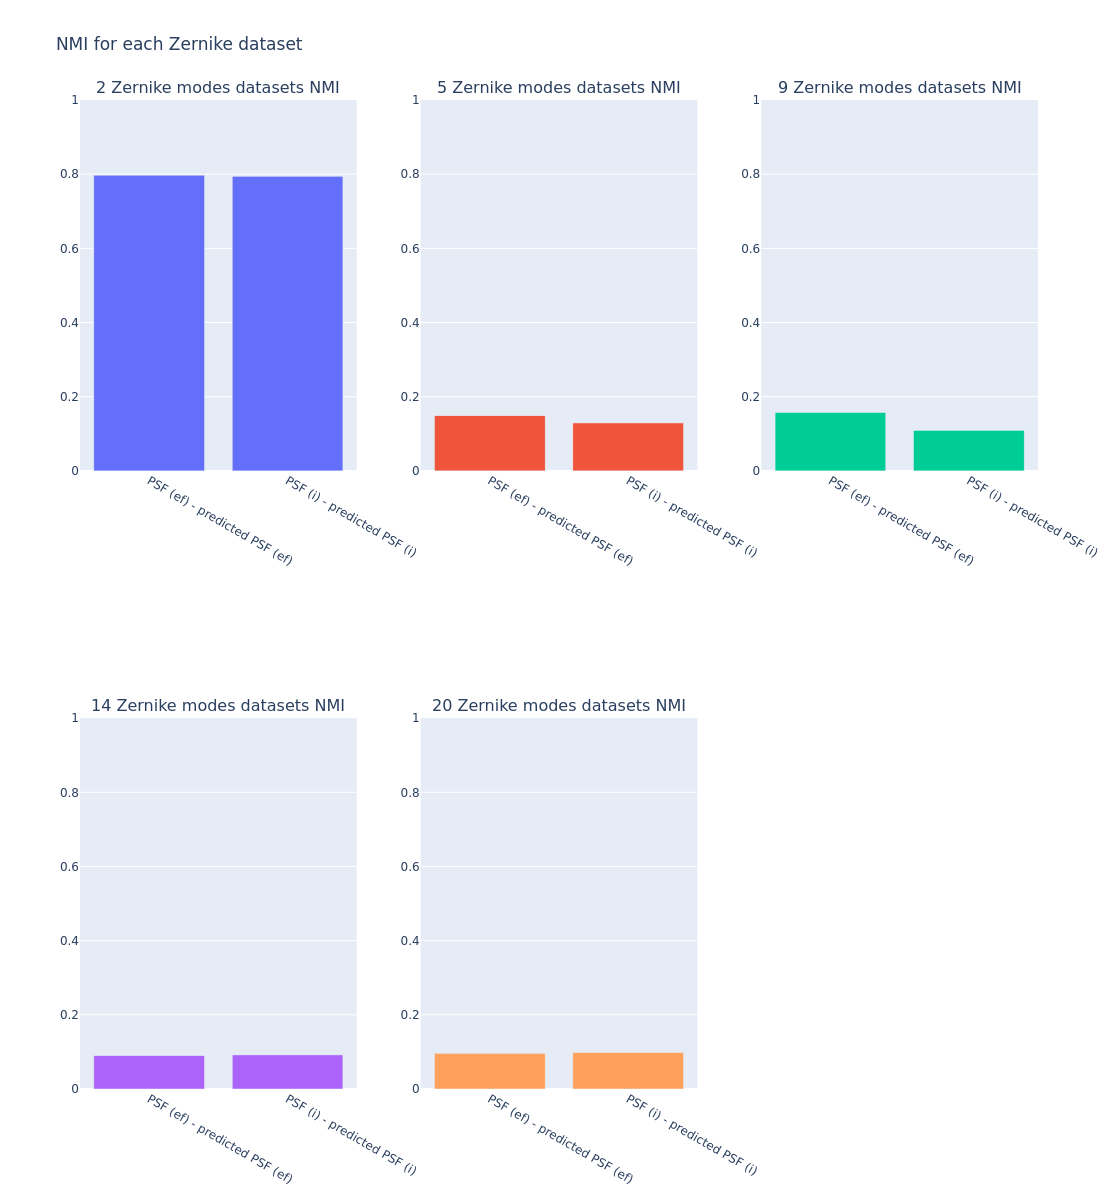
\includegraphics[width=0.9\textwidth]{pid-nmibarpsfpredpsf.png}
		\end{figure*}
		\FloatBarrier
		
		
	